\chapter{Gold Standard}
\section{Beschreibung des Gold Standards}
Der erarbeitete Gold Standard besteht insgesamt aus 6963 Dateien des Formats JSON, welche jeweils eine Webpage einer Restaurant-Website repräsentieren.
Diese Daten sind in einen Test- und einen Trainings- und Validierungsdatensatz.
Der Gold Standard ist in die folgenden drei Kategorien unterteilt:\\

\begin{forest}
	for tree={
		font=\ttfamily,
		grow'=0,
		child anchor=west,
		parent anchor=south,
		anchor=west,
		calign=first,
		edge path={
			\noexpand\path [draw, \forestoption{edge}]
			(!u.south west) +(7.5pt,0) |- node[fill,inner sep=1.25pt] {} (.child anchor)\forestoption{edge label};
		},
		before typesetting nodes={
			if n=1
			{insert before={[,phantom]}}
			{}
		},
		fit=band,
		before computing xy={l=15pt},
	}
	[Gold Standard (6963 Dateien)
	[test (100 Dateien)
	[neg (50 Dateien)]
	[pos\textunderscore daily\textunderscore menu (10 Dateien)]
	[pos\textunderscore menu (40 Dateien)]
	]
	[train-validation (6863 Dateien)
	[neg (6257 Dateien)]
	[pos\textunderscore daily\textunderscore menu (87 Dateien)]
	[pos\textunderscore menu (519 Dateien)]
	]
	]
\end{forest}\\

%\begin{tabular}{|l|l|l|l|}
%	\hline
%	Kategorie & Ordnername & Anzahl Dateien & Anzahl Dateien im Testsatz\\
%	\hline
%	Menü & pos\textunderscore menu & 519 & 40 \\
%	Tagesmenü & pos\textunderscore daily\textunderscore menu & 87 & 10 \\
%	Kein Menü & neg & 6257 & 50\\
%	\hline
%\end{tabular}\\
Jeder Eintrag dieses Gold Standards beinhaltet die folgenden Informationen:
\begin{itemize}
	\item \glqq date \grqq  - Zeitpunkt, zu welchem die Webpage aufgerufen wurde
	\item \glqq text \grqq  - Vom Webcrawler extrahierter Text, welcher die Webpage beinhaltet
	\item \glqq encoding \grqq  - Das von der Webpage verwendete Encoding
	\item \glqq title \grqq  - Inhalt des gleichnamigen HTML-Metatags
	\item \glqq url \grqq  - URL der Webpage
	\item \glqq content \grqq  - Der statische HTML-Inhalt der Webpage	
\end{itemize}
\section{Entscheidungsraster}
Der Gold Standard wurde anhand des Entscheidungsrasters erstellt, welches in der Abbildung \cref{fig:classificationtree} dargestellt wird.
\begin{figure}[H]	
	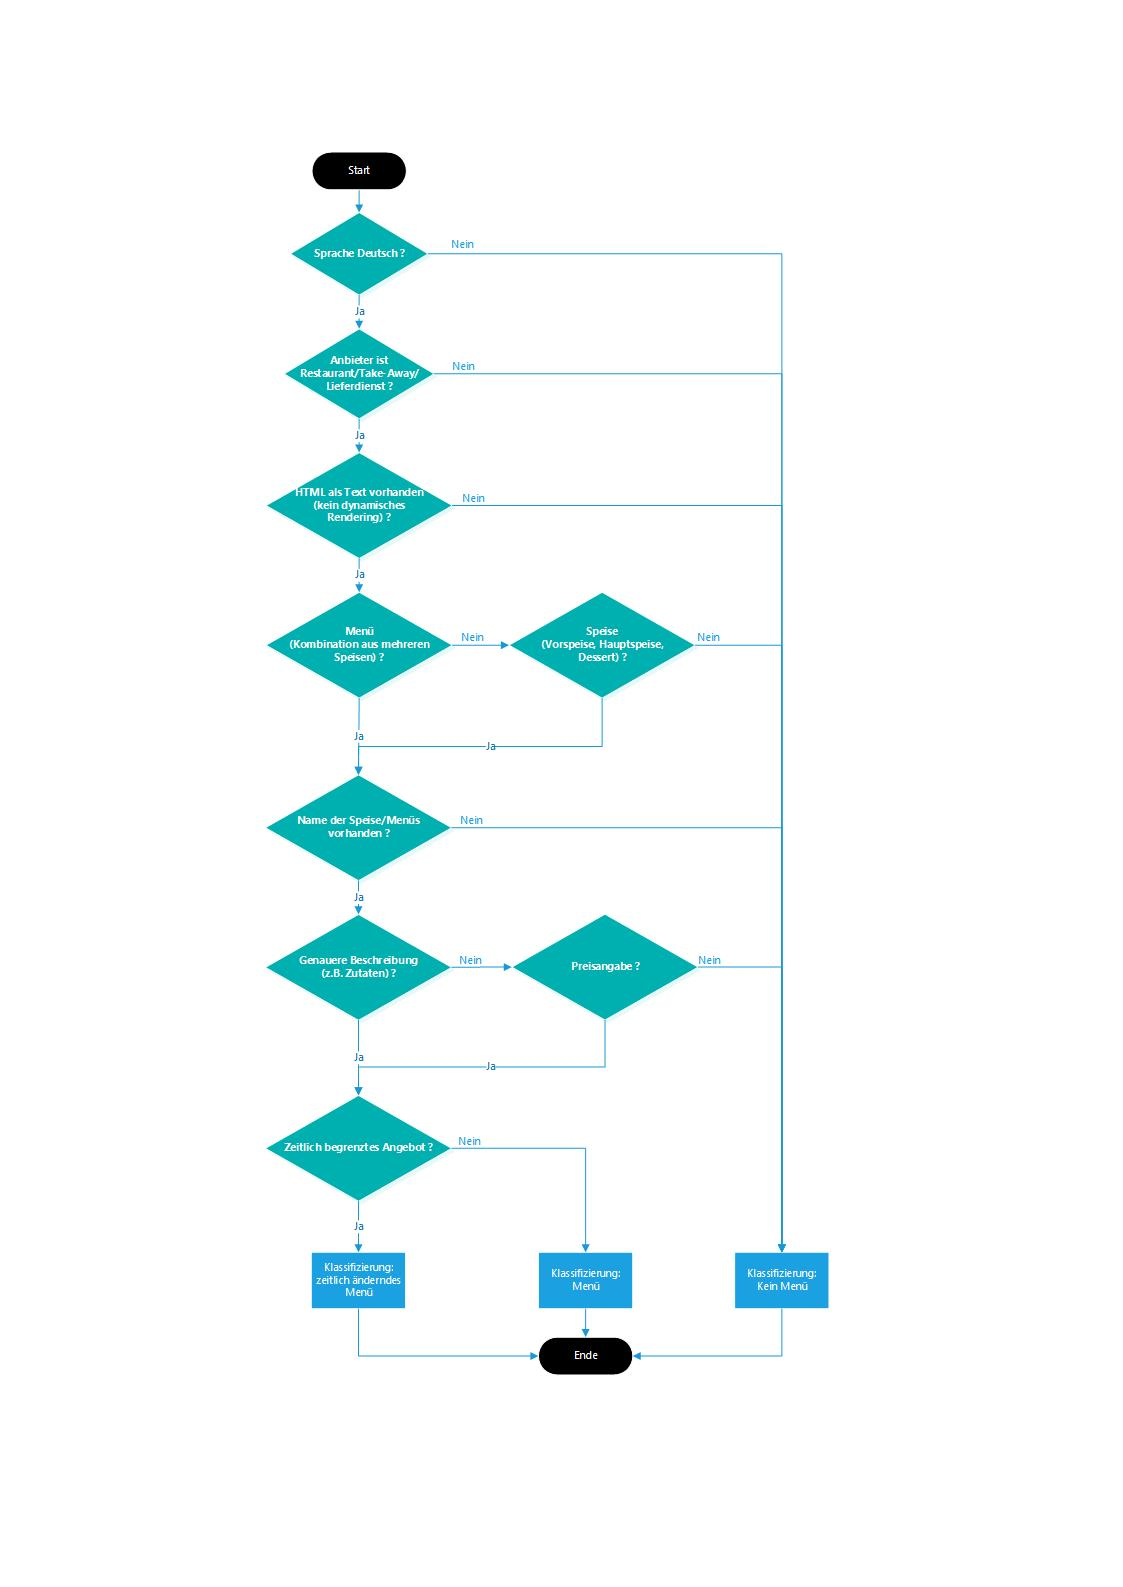
\includegraphics[width=1\columnwidth,keepaspectratio]{img/man-classification-tree.jpg}
	\caption{Entscheidungsraster}
	\label{fig:classificationtree}
\end{figure}
Obwohl bereits beim Webcrawler eine Spracherkennung eingesetzt wurde, damit nur als deutsch erkannte Webpages gespeichert werden, wurde bei der manuellen Klassifikation nochmals darauf geachtet, dass die Webpage in deutsch verfasst wurde.
Dabei ist anzumerken, dass gewisse Begriffe, vor allem für Speisebezeichnungen, auch fremdsprachig sein dürfen, da Speisebezeichnungen je nach Küche international ausgelegt sind.
Der Anbieter muss zwingend ein Restaurant, Take-Away oder Lieferdienst sein.
Der Inhalt muss als statisch verfügbar sein, da der Webcrawler nicht mit dynamisch gerenderten Websites umgehen kann.
Der Name der Speise und eine genauere Beschreibung oder der Preis muss vorhanden sein.
Danach folgt die Unterscheidung zwischen zeitlich begrenzten und unbegrenzten Angeboten, welche zur Kategorisierung führt.
Getränkekarten wurden explizit negativ klassifiziert.
\section{Seed}
Das Seed wurde aus den folgenden zwei Quellen zusammengestellt:
\begin{itemize}
	\item OpenStreetMap - 3557 URLs
	\item Lunch-Check - 3803 URls
\end{itemize}
Diese URLs wurden zusammengeführt, zudem sind Duplikate entfernt worden.
Daraus ist ein Seed entstanden, welches 5870 Einträge von Restaurant-URLs enthält.
Dabei wurden aus den nun aufgeführten Gründen mehrere Einträge entfernt:
\begin{itemize}
	\item Die Website enthält mehr als 300 Webpages
	\item Die Website ist offensichtlich keine Restaurant-Website
\end{itemize}
Websites mit mehr als 300 Webpages wurden entfernt, da diese keine typische Restaurant-Website repräsentieren und somit das Gesamtbild verzerren.
Es kann keine Gewähr gegeben werden, dass dieses Seed nur Restaurant-Websites beinhaltet, da nicht jeder Eintrag geprüft wurde.
